\chapter{Codifica}
\label{cap:codifica}

\section{Scopo del capitolo}
Nel seguente capitolo si può osservare il lavoro dei giorni seguenti alla Progettazione fino agli ultimi giorni di tirocinio. In questo capitolo viene illustrato lo sviluppo dell'API REST, come sono stati organizzati i package e le classi al loro interno, la spiegazione di frammenti di codice rilevanti ed infine una sezione per la creazione dello Swagger. \\

\section{Convenzioni di denominazione REST}
Buona prassi nella creazione di un'API REST è il rispetto di convenzioni per la nomenclatura degli endpoint. Sebbene non esista un'unica convenzione obbligatoria, esistono delle best practices\textsubscript{g} per garantire una facile lettura e comprensibilità per agevolare gli sviluppatori che adoperano l'API.\\
Le seguenti convenzioni sono state rispettate nello sviluppo dell'API:
\begin{itemize}
\item  pluralizzare le risorse, per distinguere se si fa riferimento ad una lista di una determinata risorsa o ad una singola risorsa;
\item usare lettere minuscole;
\item non usare estensioni dei file;
\item in caso di nomi composti utilizzare il "-";
\item non usare underscore;
\item non utilizzare abbreviazioni o slang;
\item non utilizzare verbi, poichè l'azione dovrebbe essere indicata dal metodo HTTP utilizzato.
\end{itemize}

\section{Verbi standard HTTP}
I verbi standard forniti da HTTP utilizzati applicati all'API REST sono i seguenti:
\setlength{\arrayrulewidth}{0.3mm}
\renewcommand{\arraystretch}{2.5}
\begin{center}
\rowcolors{1}{white}{mygray}
\begin{longtable}{p{2cm}|p{8cm}}
\textbf{Verbo}  & \textbf{Descrizione}\\
\hline
%\rowcolor{mygray} 
POST   & Utilizzato per inviare dati al server al fine di creare una nuova risorsa ed aggiungerla all'insieme corrente\\
GET    & Utilizzato per richiedere dati al server in merito ad una o più risorse senza modificarle          \\
%\rowcolor{mygray}
DELETE &   Utilizzato per eliminare una risorsa specifica dal server          \\
PUT    &   Utilizzato per aggiornare totalmente una risorsa sovrascrivendola\\
%\rowcolor{mygray}
PATCH  &     Utilizzato per effettuare aggiornamenti parziali a una risorsa esistente        \\ 
\hline
\hiderowcolors
\caption{Verbi Standard HTTP utilizzati}
\label{tab:verbi-http}
\end{longtable}
\end{center}

%Per garantire una lettura chiara dello stato dell'operazione richiesta, sono stati utilizzati i seguenti codici di risposta HTTP. Questi codici 

\section{Endpoint sviluppati}
\noindent In questa sezione si trovano le descrizioni di tutti gli endpoint implementati, suddivisi in base all'ambito di interesse. Sarà fornito anche il verbo HTTP e il percorso necessario per effettuare ciascuna richiesta.\\
\subsection*{Anagrafiche}
Questi endpoint vengono utilizzati dal Program Manager per effettuare operazioni di lettura sulle anagrafiche aziendali. 
\setlength{\arrayrulewidth}{0.3mm}
\renewcommand{\arraystretch}{2.5}
\begin{center}
\rowcolors{1}{white}{mygray}
\begin{longtable}{p{1.3cm}|p{4.95cm}|p{5.7cm}}
\textbf{Verbo}  & \textbf{Path} & \textbf{Descrizione}\\
\hline
GET    & \texttt{/area-competenza/\{id\}} & Permette la lettura di un'Area di Compentenza dato l'ID\\
GET    & \texttt{/clienti} & Permette la lettura da DB di tutti i Clienti ottenendo come risposta la lista di tutti i Clienti\\
GET    & \texttt{/clienti/\{id\}} & Permette la lettura da DB di un Cliente dato l'Id ottenendo come risposta il Cliente corrispondente\\
GET    & \texttt{/risorse/\{id\}} & Permette la lettura da DB di un Risorsa dato l'Id ottenendo come risposta la Risorsa corrispondente\\
GET    & \texttt{/ruoli} & Permette la lettura da DB di tutti i Ruoli ottenendo come risposta la lista di tutti i Ruoli\\
GET    & \texttt{/ruoli/\{id\}} & Permette la lettura da DB di un Ruolo dato l'Id ottenendo come risposta il Ruolo corrispondente\\
GET    & \texttt{/skill} & Permette la lettura da DB di tutte le Skill ottenendo come risposta la lista di tutte le Skill\\
GET    & \texttt{/skill/\{id\}} & Permette la lettura da DB di una Skill dato l'Id ottenendo come risposta la Skill corrispondente\\
\hline
\hiderowcolors
\caption{Endpoint Anagrafiche sviluppati}
\label{tab:endpoint-anagrafiche-api}
\end{longtable}
\end{center}

\subsection*{Milestones}
Questi endpoint consentono la creazione, lettura, modifica ed eliminazione di Milestones. Vengono utilizzati principalmente dal Program Manager.
\setlength{\arrayrulewidth}{0.3mm}
\renewcommand{\arraystretch}{2.5}
\begin{center}
\rowcolors{1}{white}{mygray}
\begin{longtable}{p{1.3cm}|p{4.95cm}|p{5.7cm}}
\textbf{Verbo}  & \textbf{Path} & \textbf{Descrizione}\\
\hline
POST    & \texttt{/milestones} & Permette l'inserimento di una nuova Milestone, inserendo il Progetto associato, il Commerciale, la Pianificazione e altri dettagli.\\
POST    & \texttt{/milestones/list} & Rappresenta una POST di ricerca. Restituisce una lista di Milestone in base ai filtri inseriti dall'utente, alla parola chiave inserita nella quicksearch (q) e a un booleano che determina se applicare tutti i filtri in modo congiuntivo (AND) o disgiuntivo (OR).\\
PATCH    & \texttt{/milestones/\{id\}/type} & Permette la modifica del campo Type di una Milestone su DB.\\
GET    & \texttt{/milestones/\{id\}} & Permette la lettura da DB di una Milestone dato l'Id ottenendo come risposta la Milestone corrispondente.\\
DELETE    & \texttt{/milestones/\{id\}} & Permette l'eliminazione da DB di una Milestone dato l'Id ottenendo come risposta la Milestone eliminata.\\
\hline
\hiderowcolors
\caption{Endpoint Milestones sviluppati}
\label{tab:endpoint-milestones-api}
\end{longtable}
\end{center}

\subsection*{Pianificazioni}
Questi endpoint consentono la creazione, lettura, modifica ed eliminazione di Pianificazioni.
Vengono utilizzati principalmente dal Program Manager.
\setlength{\arrayrulewidth}{0.3mm}
\renewcommand{\arraystretch}{2.5}
\begin{center}
\rowcolors{1}{white}{mygray}
\begin{longtable}{p{1.3cm}|p{4.95cm}|p{5.7cm}}
\textbf{Verbo}  & \textbf{Path} & \textbf{Descrizione}\\
\hline
GET    & \texttt{/pianificazioni/\{id\}} & Permette la lettura da DB di una Pianificazione dato l'Id ottenendo come risposta la Pianificazione corrispondente.\\
PUT & \texttt{/pianificazioni/\{id\}} & Permette la modifica parziale o totale di campi di una Pianificazione su DB sovrascrivendola.\\
DELETE    & \texttt{/pianificazioni/\{id\}} & Permette l'eliminazione da DB di una Pianificazione dato l'Id ottenendo come risposta la Pianificazione eliminata.\\
POST    & \texttt{/pianificazioni} & Permette l'inserimento di una nuova Pianificazione ed eventuali entità associate come: risorsa, ruolo, milestone, progetto, responsabile e figura.\\
POST    & \texttt/{pianificazioni/xlsx} & Permette l'esportazione di report Excel di Pianificazioni in base a filtri inseriti dall'utente.\\
POST    & \texttt{/pianificazioni/list} & Rappresenta una POST di ricerca. Restituisce una lista di Pianificazioni in base ai filtri inseriti dall'utente, alla parola chiave inserita nella quicksearch (q) e a un booleano che determina se applicare tutti i filtri in modo congiuntivo (AND) o disgiuntivo (OR).\\
PATCH    & \texttt{/pianificazioni/\{id\}/times} & Permette la modifica dei campi Data Inizio e Data Fine di una Pianificazione su DB.\\
PATCH    & \texttt{/pianificazioni/\{id\}/festivi} & Permette la modifica del campo Festivi di una Pianificazione su DB.\\
GET    & \texttt{/pianificazioni/\{id\}/audit} & Permette la lettura delle modifiche effettuate su una Pianificazione dalla tabella di log.\\
\hline
\hiderowcolors
\caption{Endpoint Pianificazioni sviluppati}
\label{tab:endpoint-pianificazioni-api}
\end{longtable}
\end{center}


\subsection*{Richieste}
Questi endpoint consentono la creazione, lettura, modifica ed eliminazione di Richieste di Pianificazioni. Vengono utilizzati principalmente dal Project Manager.
\setlength{\arrayrulewidth}{0.3mm}
\renewcommand{\arraystretch}{2.5}
\begin{center}
\rowcolors{1}{white}{mygray}
\begin{longtable}{p{1.3cm}|p{4.95cm}|p{5.7cm}}
\textbf{Verbo}  & \textbf{Path} & \textbf{Descrizione}\\
\hline
GET    & \texttt{/richieste/\{id\}} & Permette la lettura da DB di una Richiesta dato l'Id ottenendo come risposta la Richiesta corrispondente.\\
PUT    & \texttt{/richieste/\{id\}} & Permette la modifica parziale o totale di campi di una Richiesta su DB sovrascrivendola.\\
DELETE    & \texttt{/richieste/\{id\}} & Permette l'eliminazione da DB di una Richiesta dato l'Id ottenendo come risposta la Richiesta eliminata.\\
POST    & \texttt{/richieste} & Permette l'inserimento di una nuova Richiesta, inserendo le Figure Professionali e le Skill richieste e altri dettagli.\\
POST    & \texttt{/richieste/list} & Rappresenta una POST di ricerca. Restituisce una lista di Richieste in base ai filtri inseriti dall'utente, alla parola chiave inserita nella quicksearch (q) e a un booleano che determina se applicare tutti i filtri in modo congiuntivo (AND) o disgiuntivo (OR).\\
DELETE    & \texttt{/richieste/\{id\}/stato} & Permette la modifica del campo Stato di una Richiesta su DB.\\
DELETE    & \texttt{/richieste/\{id\}/priorita} & Permette la modifica del campo Priorità di una Richiesta su DB.\\
\hline
\hiderowcolors
\caption{Endpoint Richieste sviluppati}
\label{tab:endpoint-richieste-api}
\end{longtable}
\end{center}


\subsubsection*{Common}
\begin{itemize}
\item \texttt{OmiPlanException}, eccezione custom utilizzata per gestire le \textit{RuntimeException}\textsubscript{g}. Classe formata da un HttpStatus per mostrare lo stato di risposta HTTP e dal messaggio fornito al lancio dell'eccezione;
\item \texttt{PaginationDirection}, classe enum per gestire la direzione della paginazione (ASC o DESC);
\item \texttt{SortDirectionVerifierConverter}, classe che implementa l'interfaccia \textit{Converter<S,T>} (componente Java utilizzato quando si lavora con strutture dati o oggetti che devono essere trasformati o adattatati in tipi diversi) per verificare che la direzione inserita sia ASC o DESC e gestire la \textit{RunTimeException} in caso non sia una variabile enum;
\item \texttt{StringToEnumConverter}, classe che implementa l'interfaccia \textit{Converter<S,T>} per convertire la direzione Stringa inserita nell'enum della direzione di pagina.
\end{itemize}

\subsubsection*{Config}
\begin{itemize}
\item \texttt{OmiPlanExceptionHandler}, handler\textsubscript{g} con il compito di gestire le eccezioni runtime e le altre segnandole come "Unexpected error". Questa classe è annotata con \textit{@ControllerAdvice}, poiché definisce una classe che gestisce in maniera centralizzata le eccezioni. Contiene due metodi annotati con \textit{@ExceptionHandler}che gestiscono rispettivamente le \textit{RunTimeException} e le altre eccezioni generali \textit{Exception};
\item \texttt{WebConfig}, classe annotata con l'annotazione \textit{@Configuration} indicando che è una classe di configurazione e che contiene definizioni di bean o altre configurazioni necessarie per l'applicazione. Essa infatti estende \textit{WebMvcConfigurer} che consente di modificare le configurazioni predefinite di Spring MVC, in questo caso aggiungendo i converter sopra citati.
\end{itemize}

\section{Package Entities}

\begin{figure}[H] 
    \centering 
    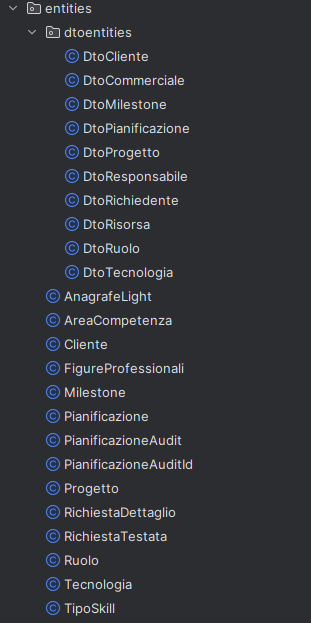
\includegraphics[width=0.4\columnwidth]{entities-package2} 
    \caption{Package entità}
\end{figure}

\noindent All'interno del package Entities troviamo le entità. Per entità si intendono tutte quelle classi Java che definiscono i modelli di dati dell'applicazione.\\
Queste classi vengono annotate con annotazioni JPA utili a stabilire come la classe venga associata a una tabella presente nel database relazionale. Ogni istanza di un'entità rappresenta una riga nella tabella relativa.\\
Di tutte le tabelle da me create è stata mappata ogni relazione tra tabelle e campo, mentre per ogni tabella del database aziendale sono stati mappati tutti i campi e le relazioni ad altre tabelle che potevano tornarmi utili.\\
In ogni entità troviamo setters e getters, costruttori con e senza argomenti.\\

\subsection{Esempio di un'entità}
\begin{figure}[H] 
    \centering 
    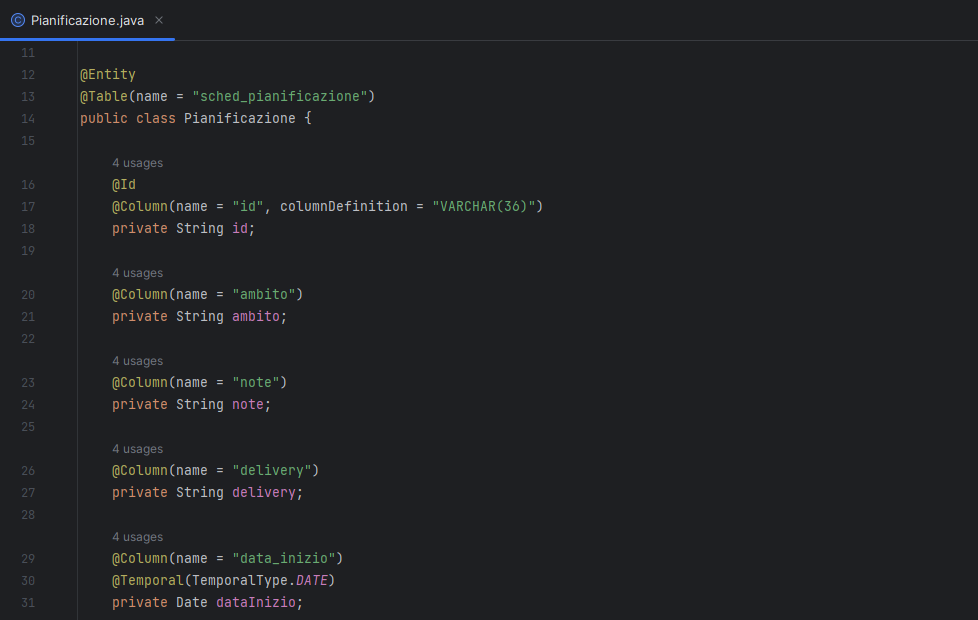
\includegraphics[width=0.9\columnwidth]{esempio-entita} 
    \caption{Esempio di mappatura di un'entità}
\end{figure}

\noindent Nell'immagine qui sopra possiamo notare uno snippet dell'entità Pianificazione in cui sono state utilizzate le seguenti annotazioni:
\begin{itemize}
\item \textit{@Entity}, per mappare le classi Java che rappresentano una tabella in un database si inserisce questa notazione specificando a class level\textsubscript{g}.
\item \textit{@Table}, nella maggior parte dei casi il nome di una tabella nel database e il nome dell'entità non sono gli stessi. Per questo motivo è stata utilizzata la seguente annotazione per specificare il nome della tabella;
\item \textit{@Column}, utilizzata per mappare una campo di una classe a una colonna di una tabella nel database. Questa annotazione possiede parametri come il "nome" per specificare il nome della colonna a cui è associato il campo;
\item \textit{@Id}, per identificare un campo all'interno di una classe come chiave primaria in una tabella del database viene utilizzata questa annotazione;
\item \textit{@Temporal}, utilizzata per specificare se un campo di tipo Date dovrebbe essere mappato come \textit{TemporalType.DATE}, per una data senza orario, \textit{TemporalType.TIME} per un orario senza data e infine \textit{TemporalType.TIMESTAMP}, utilizzato nella tabella di log di Pianificazione per mappare un campo con data e orario.
\end{itemize}
\subsection{Mappatura delle relazioni}
\begin{figure}[H] 
    \centering 
    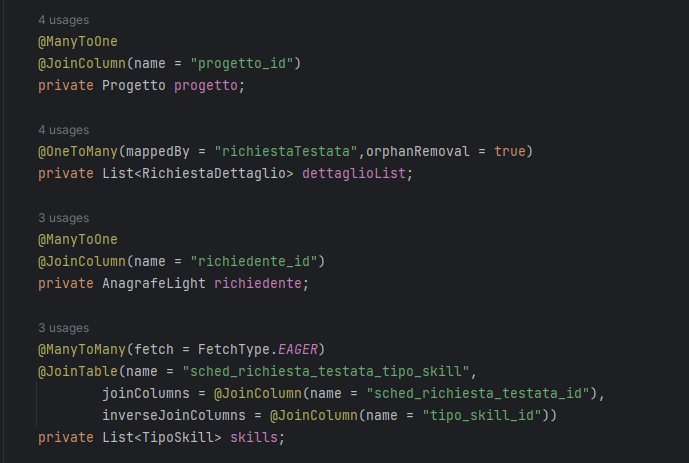
\includegraphics[width=0.9\columnwidth]{esempio-relazioni} 
    \caption{Esempio di mappatura delle relazioni della tabella RichiestaTestata}
\end{figure}
\noindent Per mantenere le relazioni tra le tabelle sono state utilizzate le annotazioni come nello snippet qui sopra raffigurante una porzione della classe Java che mappa la tabella RichiestaTestata.\\
In casi in cui entrambi i lati della relazione necessitavano per motivi implementativi, come la visualizzazione da entrambe le parti dell'informazione, di mappare la relazione opposta, veniva dichiarata una relazione bidirezionale, in cui entrambi i lati mappavano la relazione e diventava importante gestire correttamente la sincronizzazione tra le due entità.
\begin{itemize}
\item \textbf{uno-a-molti}, relazione in cui il campo associato sarà una lista di oggetti della classe opposta (in relazione all'esempio, una RichiestaTestata è associata a più RichiesteDettaglio), mentre nella relazione molti-a-uno sarà un oggetto singolo della classe opposta annotato con \textit{@JoinColumn} con \texttt{name} uguale a quello del campo nella tabella del database (in relazione all'esempio, una RichiestaTestata ha un solo Richiedente).\\
Nell'esempio è stato utilizzato il parametro \texttt{mappedBy} per mappare la relazione opposta e \texttt{orphanRemoval} per poter implementare la cancellazione di una RichiestaTestata garantendo l'eliminazione di tutte le RichiesteDettaglio associate al momento della rimozione.
\item \textbf{uno-a-uno}, relazione in cui un record della tabella è associato ad un solo record dell'altra tabella. Anche in questo caso se si vuole mappare da entrambi le parti la relazione bisogna utilizzare lo stesso principio dichiarato nella relazione \textit{@OneToMany}, solo che da entrambi le parti avranno come campo un oggetto della classe opposta.\\
Non sono state identificate relazioni uno-a-uno nel database.
\item \textbf{molti-a-molti}, relazione in cui viene mappata la tabella di join presente nel database tra le due tabelle, utilizzando il codice che si vede in esempio.
Per gestire operazioni di rimozione tra le due tabelle è stato utilizzato un metodo annotato con \textit{@PreRemove} nella classe TipoSkill, che entra in azione quando una RichiestaTestata viene eliminata, assicurando che la disconnessione avvenga in modo appropriato.
%\item \textbf{relazione bidirezionale}, relazione in cui è importante gestire correttamente la sincronizzazione tra le due direzioni della relazione, dato che quando si aggiorna una parte dell'entità bisogna aggiornare anche l'altra. Per mappare una relazione non è necessario mappare entrambi i lati della relazione, ma ritorna utile solo in base quello che si va ad implementare.
\end{itemize}
\subsection{Subpackage dtoentities}
All'interno del package "dtoentities" troviamo tutte quelle classi DTO delle entità di cui servivano soltanto determinate informazioni da restituire all'utente, evitando così ridondanza o informazioni superflue. Queste classi non contengono annotazioni, ma sono semplicemente degli oggetti contenenti i campi semplificati delle entità. A loro volta possono contenere altri DTO di altre entità in base alle relazioni che hanno.
\begin{figure}[H] 
    \centering 
    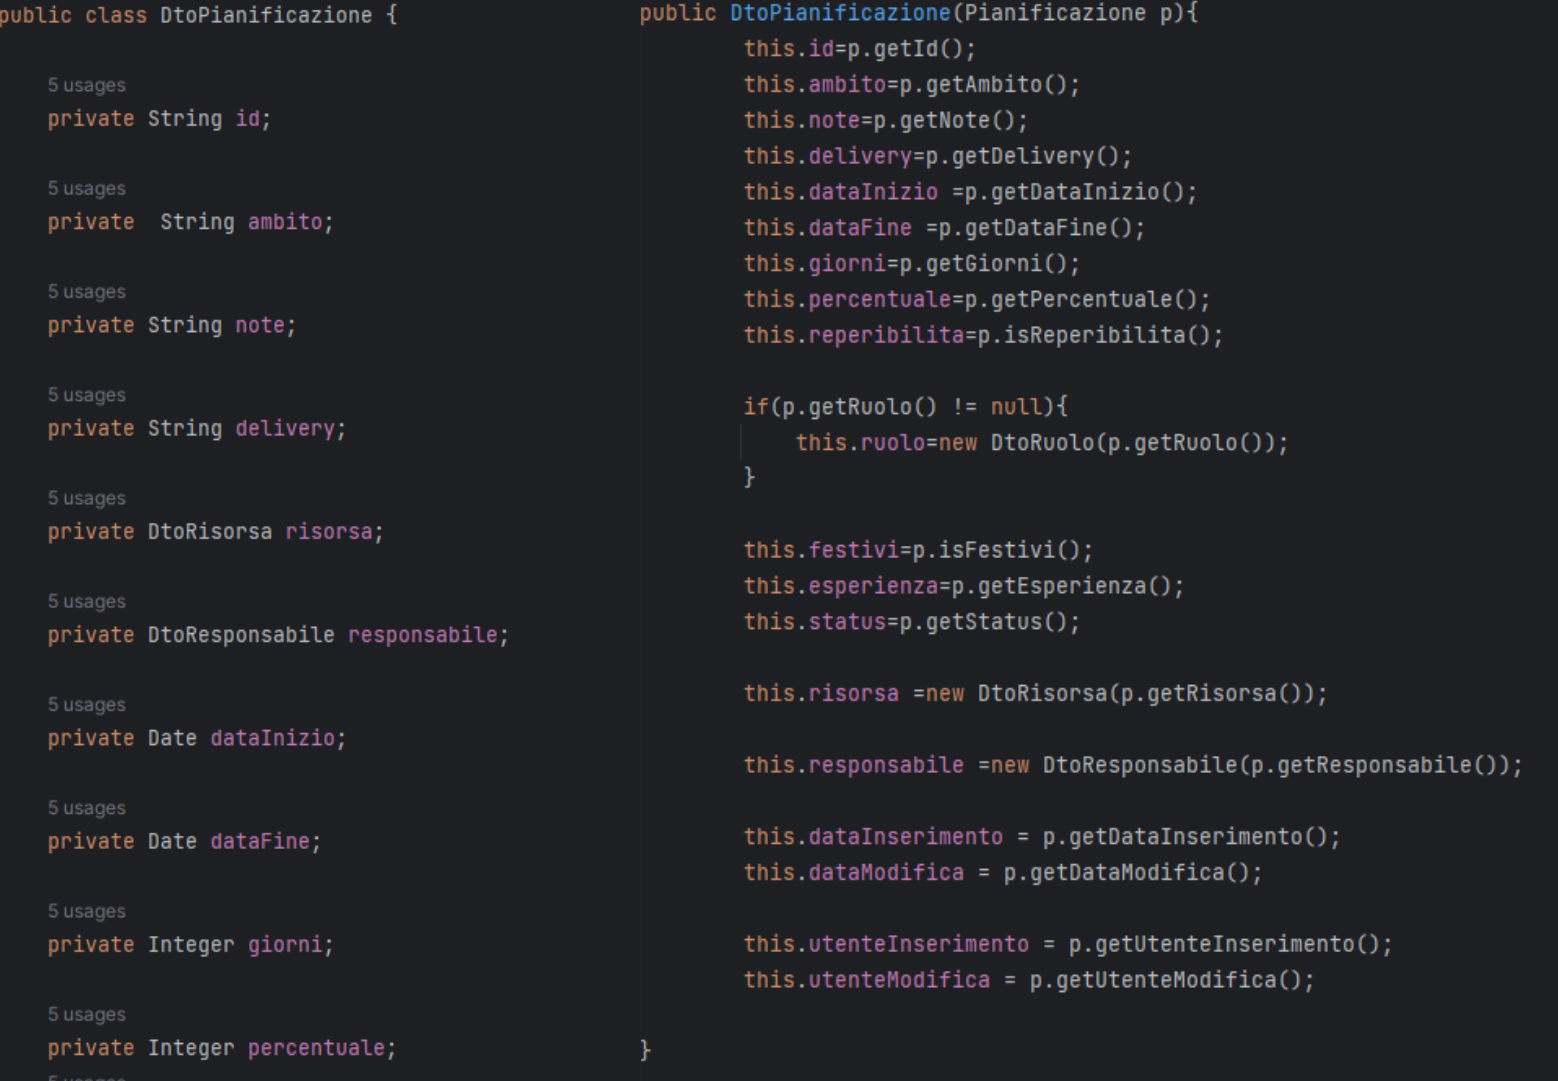
\includegraphics[width=0.9\columnwidth]{merge-dtopianificazione} 
    \caption{Esempio di classe DTO di Pianificazione}
\end{figure}
\noindent Ogni entità DTO possiede tre costruttori: costruttore senza argomenti e con argomenti e infine un costruttore che velocizzava la conversione da entità ad entità DTO (come mostrato nell'immagine qui sopra).

\section{Package dto}
Per la composizione delle richieste che il client invia o delle risposte che il server manda, sono state create vari tipi di requests e responses.\\
Ogni oggetto di risposta è composto da un oggetto "data" e un oggetto "metadata", mentre gli oggetti di richiesta possono variare. Se la richiesta è costruita per un endpoint che restituisce una lista di risultati, possiamo avere due casistiche:
\begin{itemize}
\item corpo della richiesta (body) formato da un oggetto "data", contenente informazioni utili alla risposta, e "metadata" che contiene i dati di paginazione;
\item nessun corpo, ma soltanto i dati di paginazione passati come parametri di query\textsubscript{g}.
\end{itemize}
Se invece la richiesta è costruita per un endpoint che restituisce un singolo oggetto nell'oggetto data, non viene utilizzato alcun body o parametri di query, ma solo una path variable.\\
Questa suddivisione "data" e "metadata" è un modello comune nella progettazione API per separare i dati effettivi o dati che forniscono informazioni per ottenere un tipo di risposta, dalle informazioni aggiuntive che descrivono il risultato o aggiungono caratteristiche alla richiesta.\\
Questo package è formato da vari subpackage.
\subsection{Common}
\begin{figure}[H] 
    \centering 
    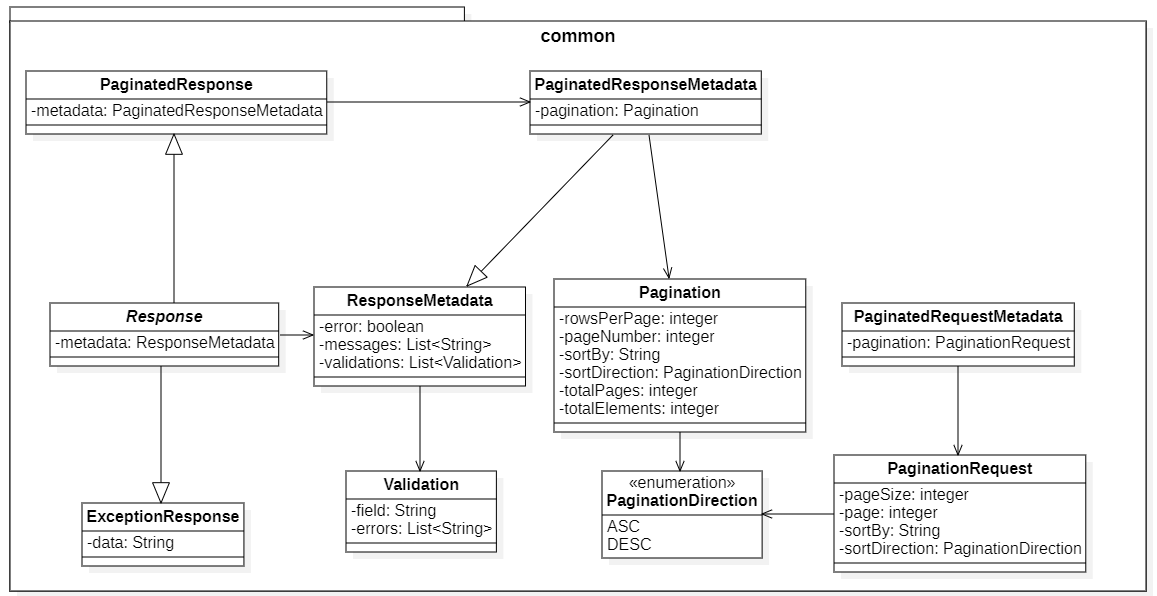
\includegraphics[width=1.0\columnwidth]{dto-sub-common} 
    \caption{Subpackage common}
\end{figure}
Questo subpackage contiene la response di base, response paginata, la response utilizzata nell'eccezione personalizzata, una request per la paginazione e i vari metadata utilizzati nelle responses.\\ Ogni \texttt{Metadata} contiene un boolean che indica se si è andati in errore (true) o meno (false), il messaggio di errore e una lista di \texttt{Validation}, contenente informazioni di validazione dei dati.\\
Ogni \texttt{Response} verrà poi estesa dalle classi che costituiscono le risposte ritornate per entità nel subpackage Responses.\\
È stata inoltre creata una classe \texttt{Pagination} per avere un controllo personalizzato sulla Paginazione.
\subsection{Requests e Body}
\begin{figure}[H] 
    \centering 
    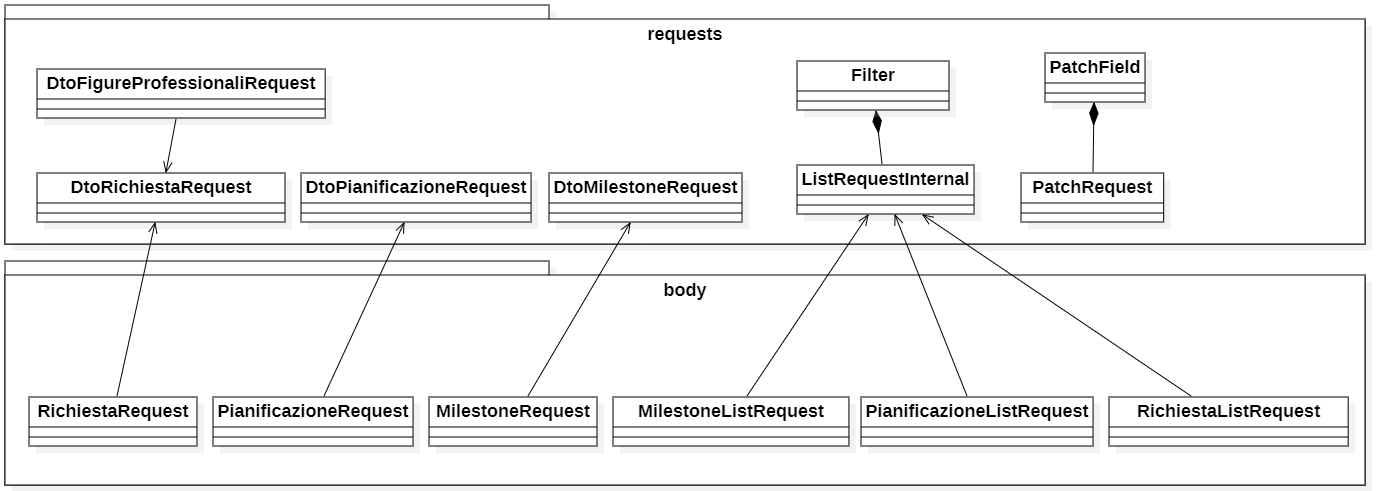
\includegraphics[width=1.0\columnwidth]{dto-sub-requests-body-2} 
    \caption{Subpackage requests e body}
\end{figure}
Questi due subpackages sono correlati tra di loro dato che ogni body ha come attributo una request presa dal subpackage requests.
Esistono due tipi di body:
\begin{itemize}
\item ogni \texttt{Request} singola è utilizzata per richiedere una specifica risorsa e contiene una request DTO formata dai campi utili che l'utente deve inserire;
\item ogni \texttt{ListRequest} è utilizzata per richiedere una o più risorse ed è formata da un oggetto data di tipo \texttt{ListRequestInternal}, che contiene tre parametri:
\begin{itemize}
\item filters, lista di oggetti \texttt{Filter} formati da campo-valore;
\item una stringa q (quicksearch) utile nella query personalizzata per cercare in determinati campi quello che l'utente inserisce;
\item andOperator per impostare i filtri in And o in Or nella query.
\end{itemize} 
\end{itemize}
All'interno del subpackage requests troviamo anche \texttt{PatchRequest}, contenente un unico campo corrispondente ad una lista di \texttt{PatchField}. Questa richiesta viene utilizzata nella richieste PATCH, in cui è possibile inserire uno o più valori in base a cosa si va a modificare.

\subsection{Responses}
\begin{figure}[H] 
    \centering 
    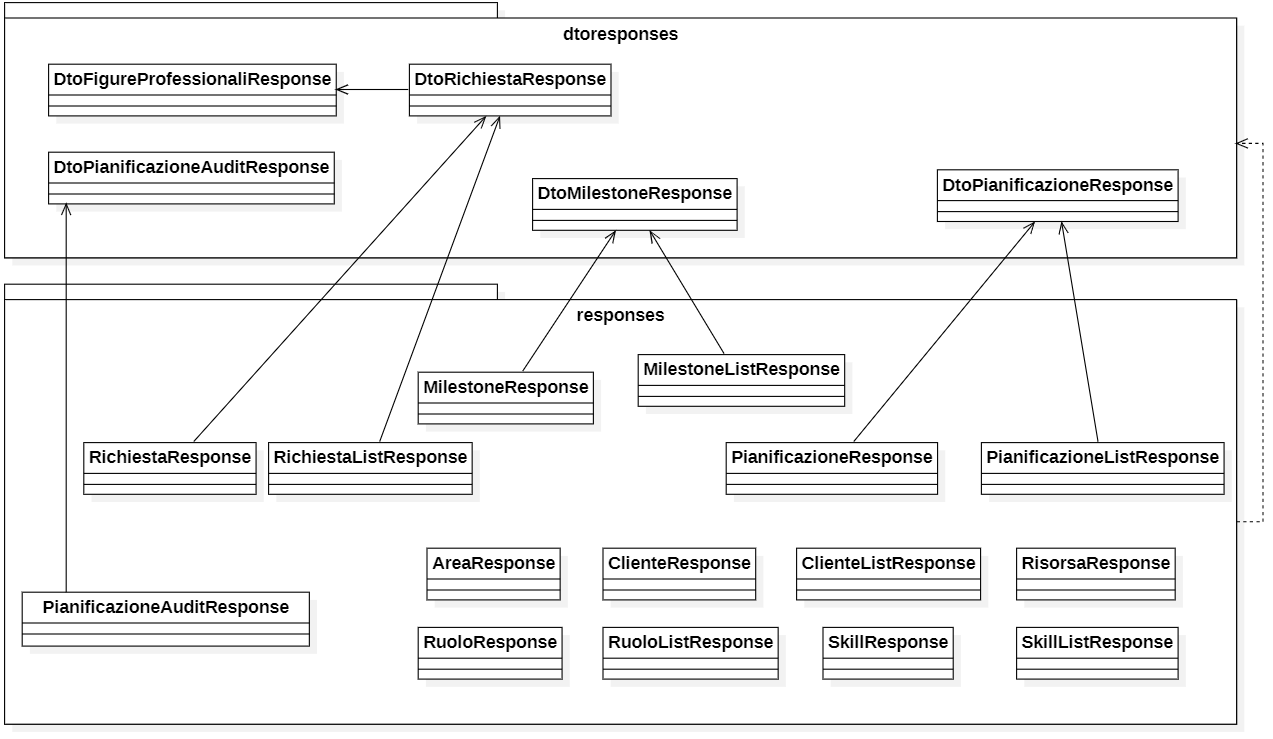
\includegraphics[width=0.9\columnwidth]{dto-sub-responses} 
    \caption{Subpackage responses e dtoresponses}
\end{figure}
Il package responses contiene tutte le response per entità. Ogni response estende la classe astratta \texttt{Response} se è una risposta singola, altrimenti estende la classe \texttt{PaginatedResponse} se è una lista di risposte. Questo permette all'utente di visualizzare la risposta, dopo aver interagito con un'endpoint, formata da "data" e "metadata".\\
Ogni response contiene un solo attributo che corrisponde all'oggetto "data" e può essere:
\begin{itemize}
\item una response DTO del subpackage dtoresponses;
\item un'entità DTO del subpackage delle entità;
\item in caso di una \texttt{ListResponse} l'attributo sarà una lista di response.
\end{itemize}

\subsection{Repository-Service-Controller}

\begin{figure}[H] 
    \centering 
    \includegraphics[width=0.85\columnwidth]{csp_img} 
    \caption{Schema di collegamento tra i componenti Repository,Service e Controller}
\end{figure}

\noindent Funzionamento.\\

\noindent \texttt{FOTO DI COME SONO NELLA DIRECTORY}\\

\noindent Presentazione di una Repository in particolare con spiegazione annotazioni.\\\\
Presentazione di una Service in particolare con spiegazione di un metodo in particolare, magari quello che excell che esegue la query.\\\\
Presentazione di un ControllerImpl in particolare con spiegazione annotazioni.\\\\

\subsection{Swagger UI}
Spiegazione come è stata creata la grafica per gli endpoint con screen di un'interfaccia Controller.

\section{Generazione automatica dello Swagger}
Per creare la documentazione dell'API è stata utilizzata la dipendenza \textit{springdoc-openapi-starter-webmvc-ui} citata nella sotto-sezione \hyperlink{doc-api}{4.7.2.1} nel capitolo di Progettazione. Grazie a questa dipendenza è stato possibile generare automaticamente la documentazione dell'API basata sulle annotazioni presenti nel codice sorgente. SpringDoc API utilizza le annotazioni di Spring per identificare i Controller, i metodi delle API, i dati in input e in output. Per visualizzare questo documento generato è possibile accederci tramite un endpoint specifico: \textit{https://localhost:porta\_scelta/swagger-ui.html}.
\begin{figure}[H] 
    \centering 
    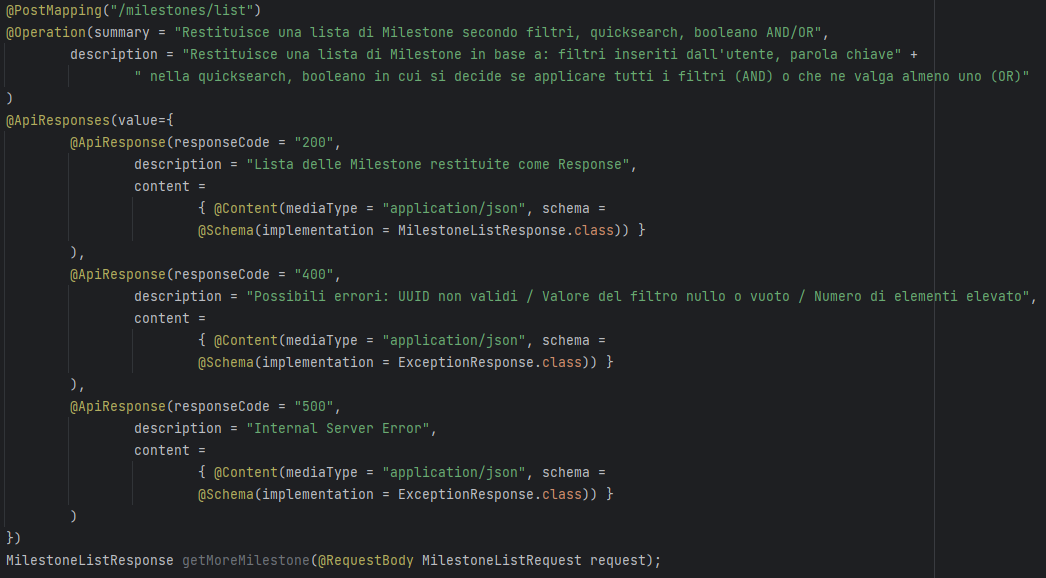
\includegraphics[width=0.90\columnwidth]{api-doc-annotazioni} 
    \caption{Annotazioni utili a generare la documentazione per l'API}
\end{figure}
\noindent La dipendenza importata fornisce anche annotazioni per arrichire il documento. In questa immagine notiamo le seguenti annotazioni:
\begin{itemize}
\item \textit{@Operation}, specifica un sommario dell'endpoint che l'utente può vedere prima di visualizzare nella sua totalità l'endpoint e un campo descrizione per fornire una descrizione più approfondita sul funzionamento;
\item \textit{@ApiResponses}, formata da tanti \textit{@ApiResponse} che specificano il codice di errore, la descrizione di quando questo errore esce e lo schema che avrà quando si presenterà.
\end{itemize}
Per agevolare la lettura dell'API è stata anche utilizzata la notazione \textit{@Schema} per fornire un nome appropriato a campi o classi.







